\section{Oscilloscope side}
    \subsection{Server} The server is responsible for receiving the messages containing the outcome instances from the adapter. The server forwards the instances to the oscilloscope.
    
    \subsection{$\Delta$Q Oscilloscope} The oscilloscope is a C++ graphical application which implements a dashboard to observe $\Delta$Qs of probes inserted in the system under test \cite{osc-g}. It receives the instances corresponding to probes from the server and adds them to the time series of the probes whose instance is being received. 
    The oscilloscope has a graphical interface which allows the user to create an outcome diagram of the system under test, display real time graphs which show detail about the execution of the system and allow the user to set parameters for probes. It can also display snapshots of the system as if it was frozen in time.

    \subsection{Inserting probes in the oscilloscope}
        Probes are automatically inserted in the oscilloscope when creating outcome diagrams. They are inserted on the outcomes observables, operators observables and to the sub-outcome diagrams observables (probes that observe the causal links of multiple outcomes/operators), we will see later on how they can be defined and how an outcome diagram can be created. \\
    The names that are given to outcome, operators and sub-outcome diagrams are the names of the probes that observe them. Giving these probes a name allows the oscilloscope to match the outcome instances received by the adapter to the probes' time series.

        In the system below (\cref{fig:probes_o}), which is equal to the one defined previously (\cref{fig:probes}), probes are automatically attached to outcomes $o_1, o_2$. The user who wants to observe the result of the sequential composition can insert probes at the start and end of the routine. 
    
        \begin{figure}[H]
            \begin{center}
                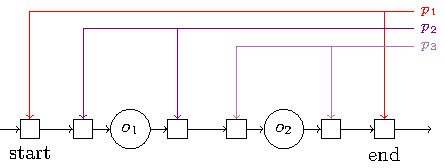
\includegraphics[scale=1.3]{tikz/probe_1.pdf}
            \end{center}
            \caption{Probes inserted in the outcome diagram of the previous component diagram in \cref{fig:probes}.}
            \label{fig:probes_o}
        \end{figure}
       
    The \textbf{observables} are an abstract representation of events. Consider the previous code snippet \cref{code:adapter}: the $start$ event of ``probe'' and worker$_1$'s start event are subsequent instructions. The probe's start event is practically the same as worker$_1$'s start event, indeed, they could be overlapped in the graph above (\cref{fig:probes_o}). We nevertheless show the distinction to show that probe and worker$_1$ need to be started differently in Erlang as the information they carry is about two distinct instances. It is the same concept as starting a parent/child span. Furthermore, this difference is remarked in the definition of outcome diagrams for the oscilloscope, for which we provide a syntax in the Chapter 4. 
    
    As for operators, probes are automatically attached to the components inside them and to the operators' observables (\cref{fig:probes_op}). 

       \begin{figure}[H]
           \begin{center}
                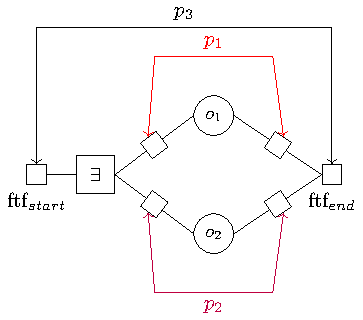
\includegraphics[scale = 1.3]{tikz/probe_2.pdf}
            \end{center}
            \label{fig:probes_op}
            \caption{Probes inserted into an operator.}
       \end{figure}
    
    The \textbf{observed $\Delta$Q} for the first-to-finish operator is the$\Delta$Q for the observables (\textbf{start}, \textbf{end}). The \textbf{calculated $\Delta$Q} is the $\Delta$Q which is the result of the first-to-finish operator being applied on $o_1, o_2$.
